\documentclass[12pt]{scrartcl}
\usepackage{geometry}
\usepackage{amsmath}
\usepackage[english]{babel}
\usepackage{fontspec}
\usepackage{hyperref}
\setmainfont{Liberation Serif}
\geometry{a4paper,left=30mm,right=30mm, top=2cm, bottom=2cm}

\begin{document}
  \title{Project Work at MPIK}
  \subtitle{Temperature control system}
  \date{}
  \author{Stefan Dickopf}
  \maketitle

  \section{Experimental setup}
    A temperature sensor, a heater and a cooler are to be connected to a Arduino
    board. In order for it to work we need to have shifters for the voltage
    range to fit the inputs/outputs on the Arduino. This was first done by
    Vanessa Scheller using cables and a breadboard, I took her design and
    reworked it to be used on a milled circuit board and SMD parts.

    \subsection{Temperature sensor circuit}
      The circuit for the temperature sensor looks as follows:
      \begin{figure}[h]
        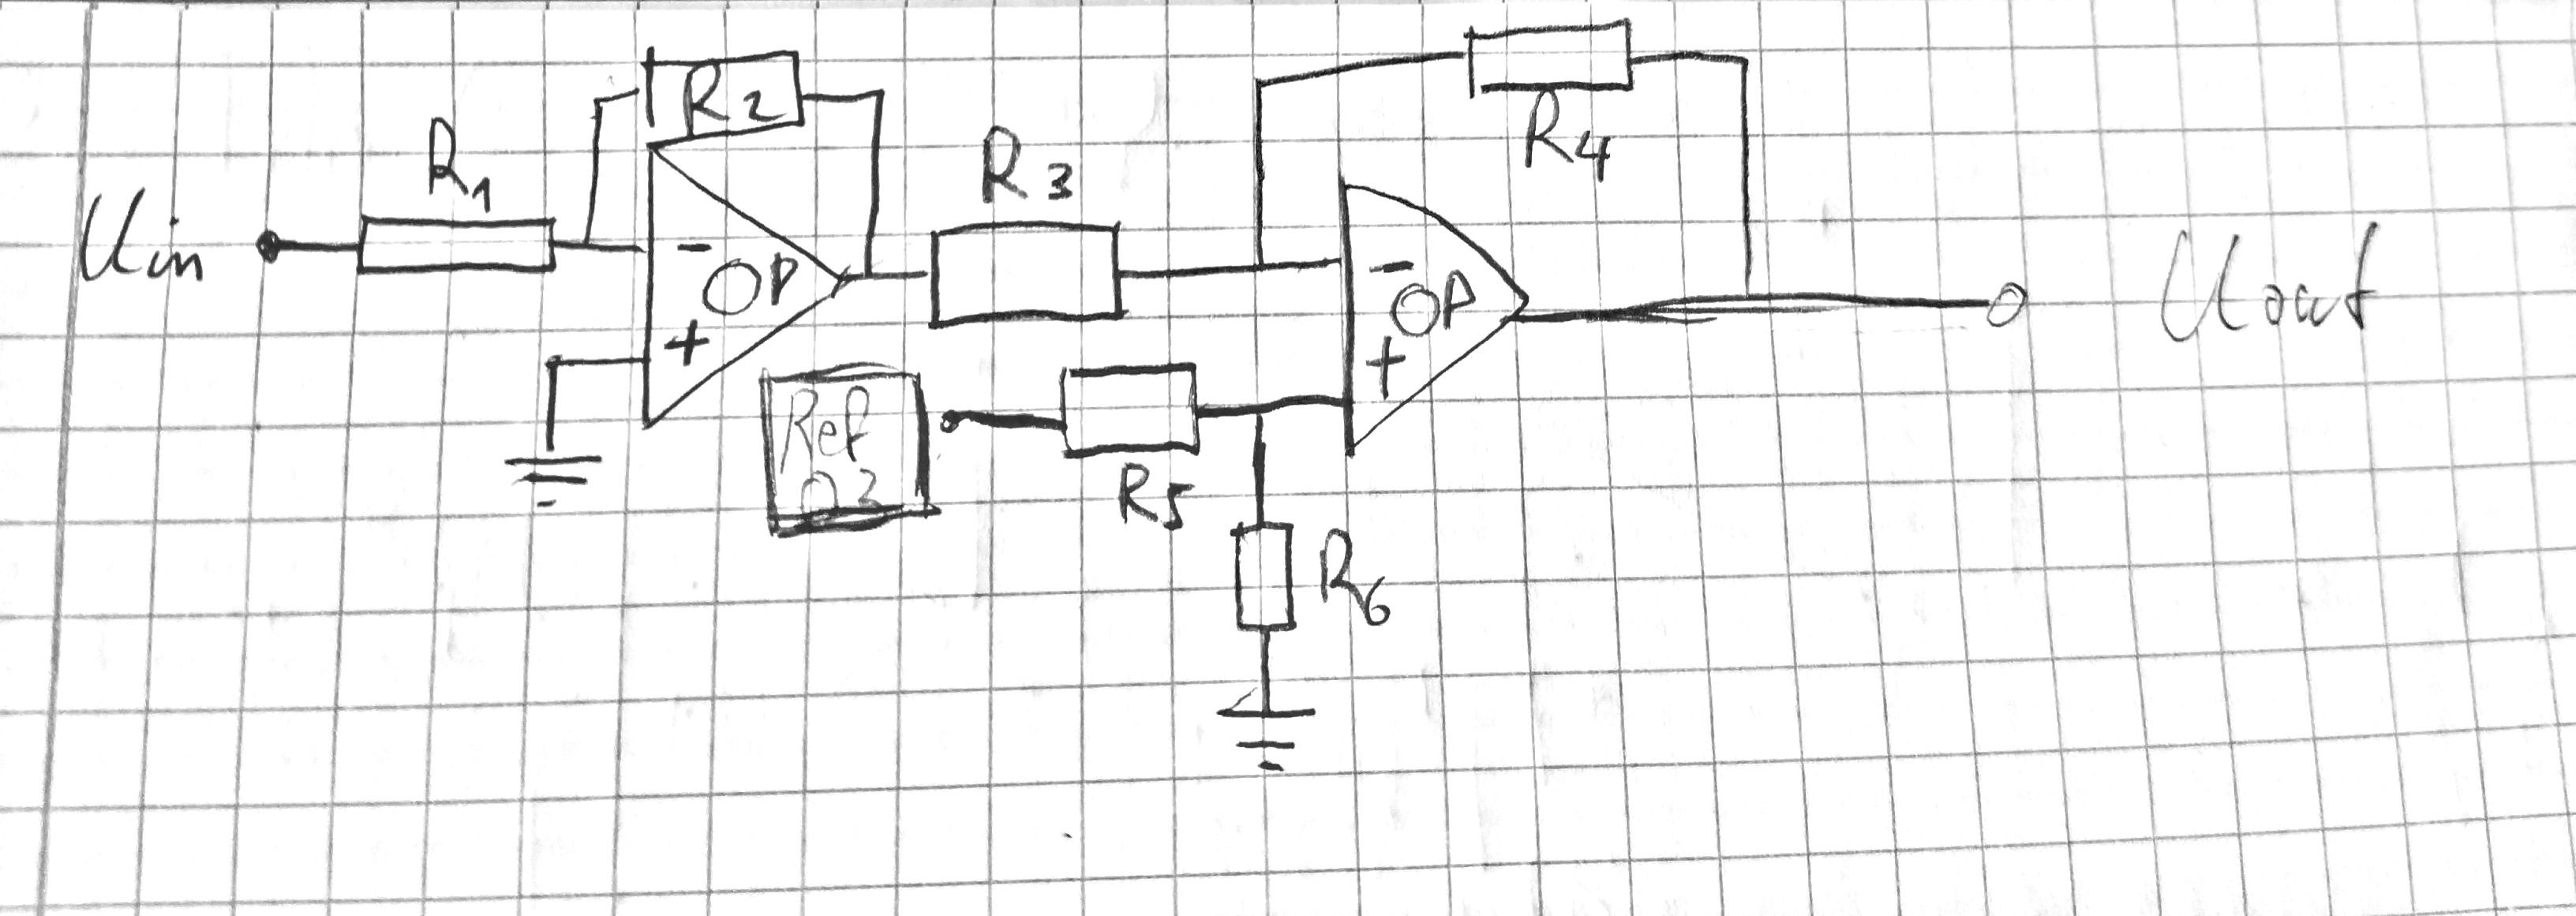
\includegraphics[width = \textwidth]{circ.png}
        \caption{Temp. sensor shifter circuit}
        \label{fig1}
      \end{figure}
      \\The input range from the temperature sensor we are interested in is
      $$-1.6V < U_{in} < 1.6V$$
      The supply voltage of the op-amps is 15V. We want to have a cutoff after
      the first op-amp at the input range boundaries. This can be achieved with
      setting the amplification factor with $R_1$ and $R_2$. The output range
      should equal the input range of the Arduino analogue input which goes form
      0-3.3V. The values found for the resistances are as follows (in $k\Omega$):
      \\
      $R_1 = 15k\Omega$ \\ $R_2 = 133k\Omega$ \\ $R_3 = 133k\Omega$ \\
      $R_4 = 12k\Omega + 10k\Omega$\text{ potentiometer} \\ $R_5 = 10k\Omega$ \\
      $R_6 = 15k\Omega + 5k\Omega$\text{ potentiometer} \\
      \\This gives to following response to the input Voltage $U_{in}$\\
      \begin{figure}[h]
        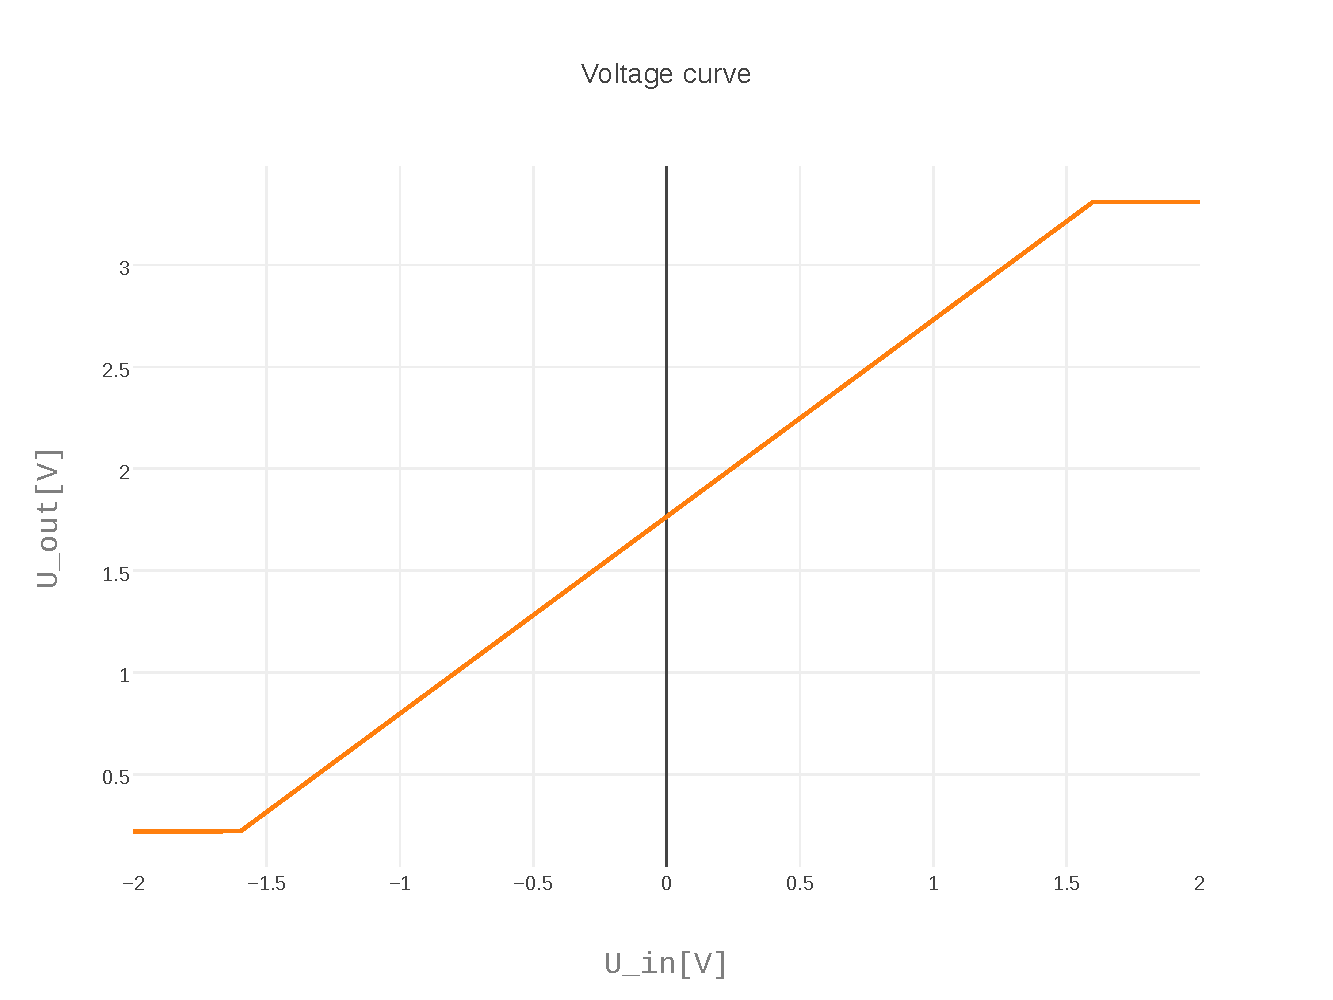
\includegraphics[width = \textwidth]{./plots/plot_image.pdf}
        \caption{Theoretical response of temp. shifter}
        \label{fig2}
      \end{figure}

    \subsection{Heater, cooler circuit}
      \begin{figure}[h]
        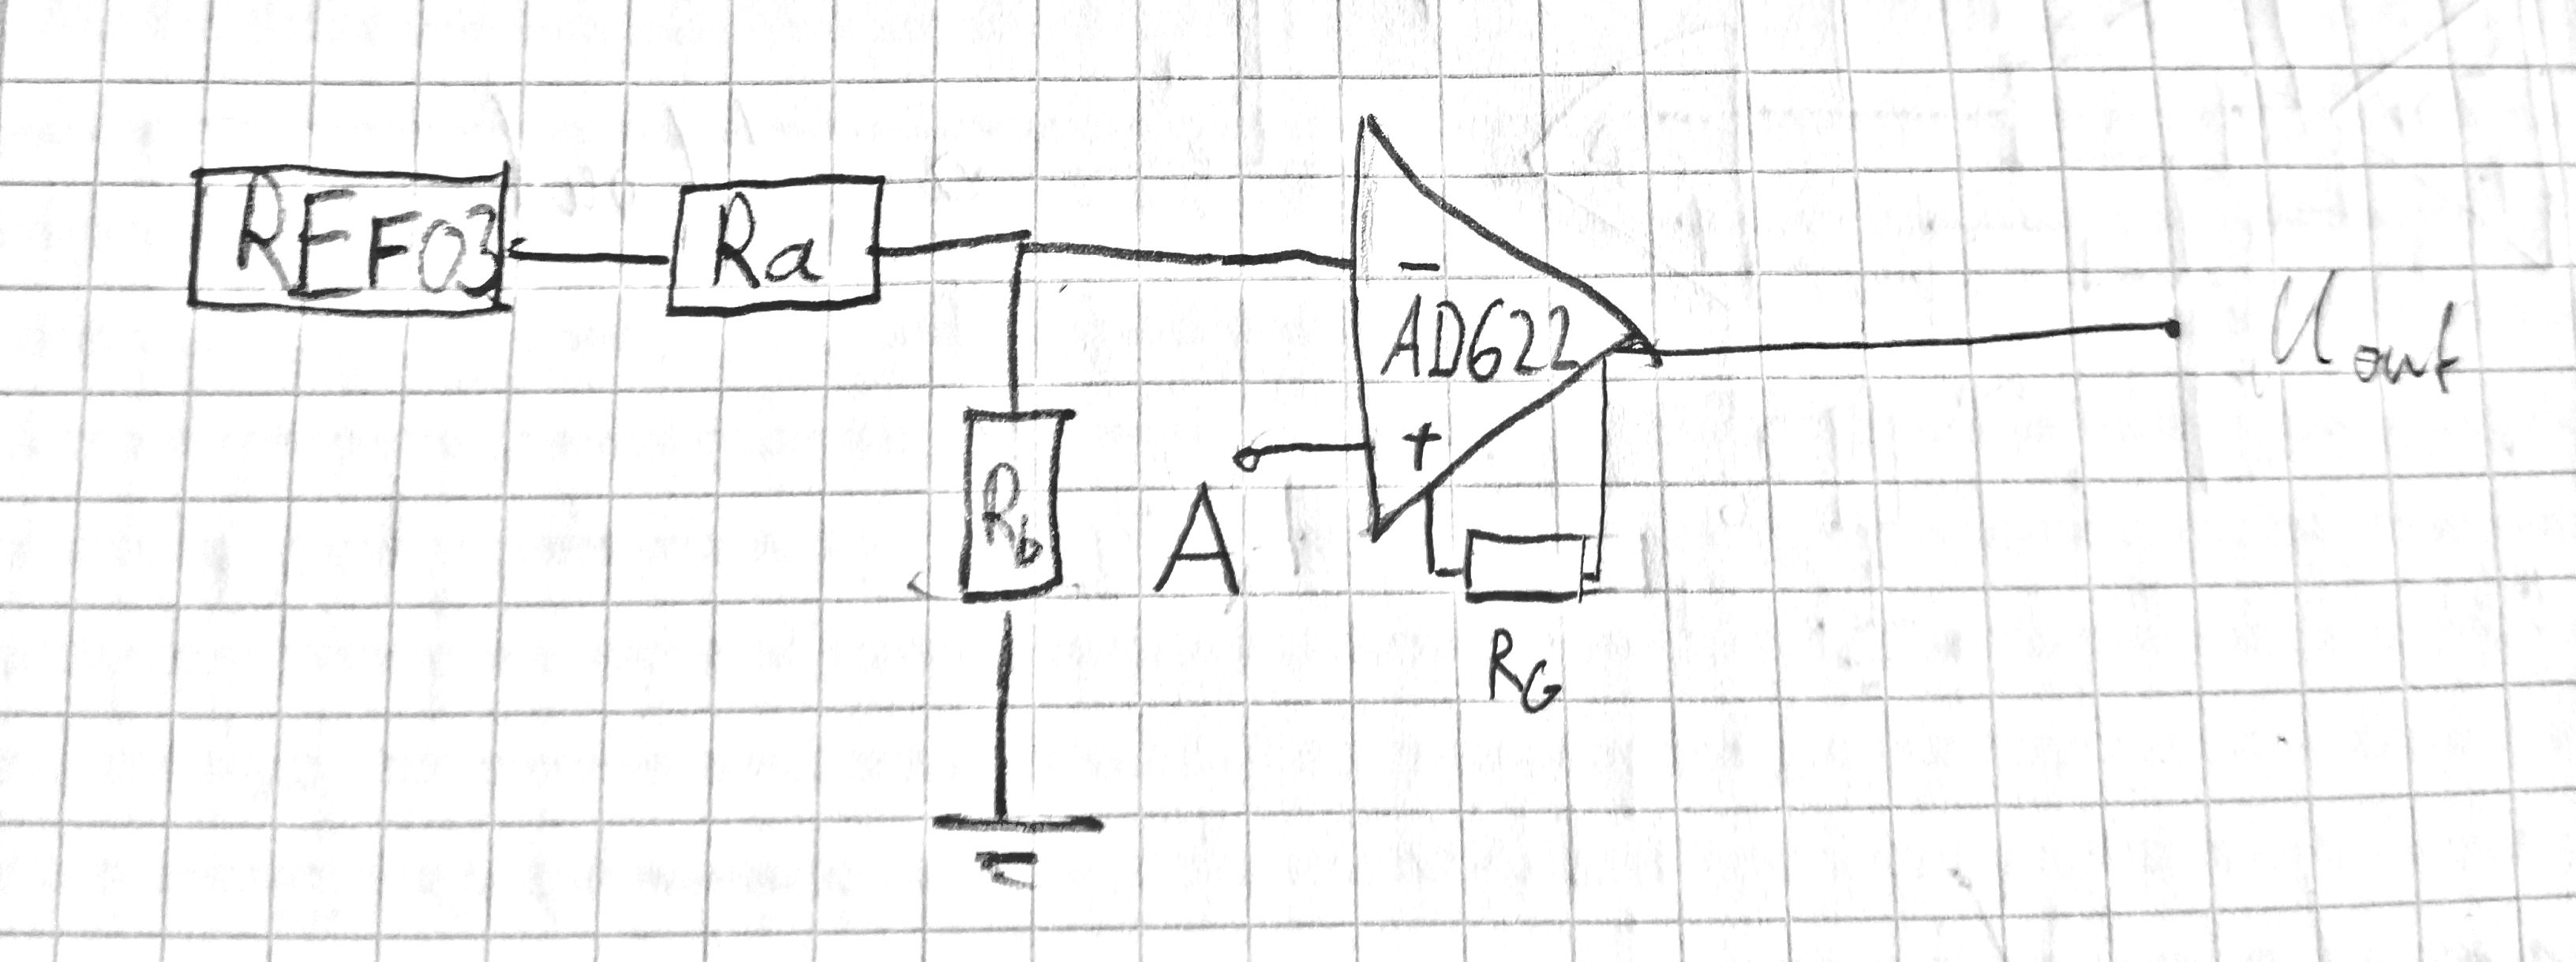
\includegraphics[width = \textwidth]{circ2.png}
        \caption{Heater/cooler shifter circuit}
        \label{fig3}
      \end{figure}
      The output range from the Arduino's DAC is $$0.55V < U_{DAC} < 2.75V$$
      The regulation voltage from the heater and cooler is 0 to 10V. First the
      voltage from the DAC out needs to be reduced by 0.55V and then amplified
      such that the maximum out from the DAC corresponds to the maximum in from
      the heater/cooler. The amplification is set with the resistance RG.
      The values found by Vanessa are (in $k\Omega$): \\
      $R_a = 3.92k\Omega + 5k\Omega$\text{ potentiometer} \\ $R_b = 1k\Omega$ \\
      $R_G = 27k\Omega + 10k\Omega$\text{ potentiometer} \\ \\
      The output here can be described by the amplified difference of the two
      input voltages. The amplification factor was adjusted such that it gives
      the needed output range.
      To both circuits many capacitances are added, which are only for filtering
      the input +15V/-15V and the ref03 voltages from AC parts. This is done with
      10nF and 100nF capacitances in parallel.

    \subsection{Realization of the circuitboard}
      All of the circuits were realized using a smd board. The circuitboard was
      constructed using EAGLE Professional and made with a circuit board cutter.
      It has the same proportions as the used arduino due, such that it fits
      into the enclosure thats already existing.
      \begin{figure}[h]
        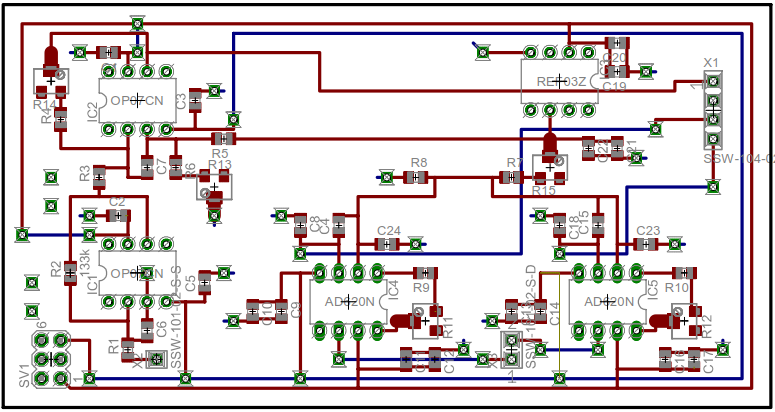
\includegraphics[width = \textwidth]{board.png}
        \caption{Circuitboard layout}
        \label{fig4}
      \end{figure}
      \\The resistors and the capacitances are directly soldered onto the board,
      while the OP07 and the AD622 (not 620 as on the image) are put onto
      headers. The complete board is shown here in fig. \ref{fig5}.
      \begin{figure}[h]
        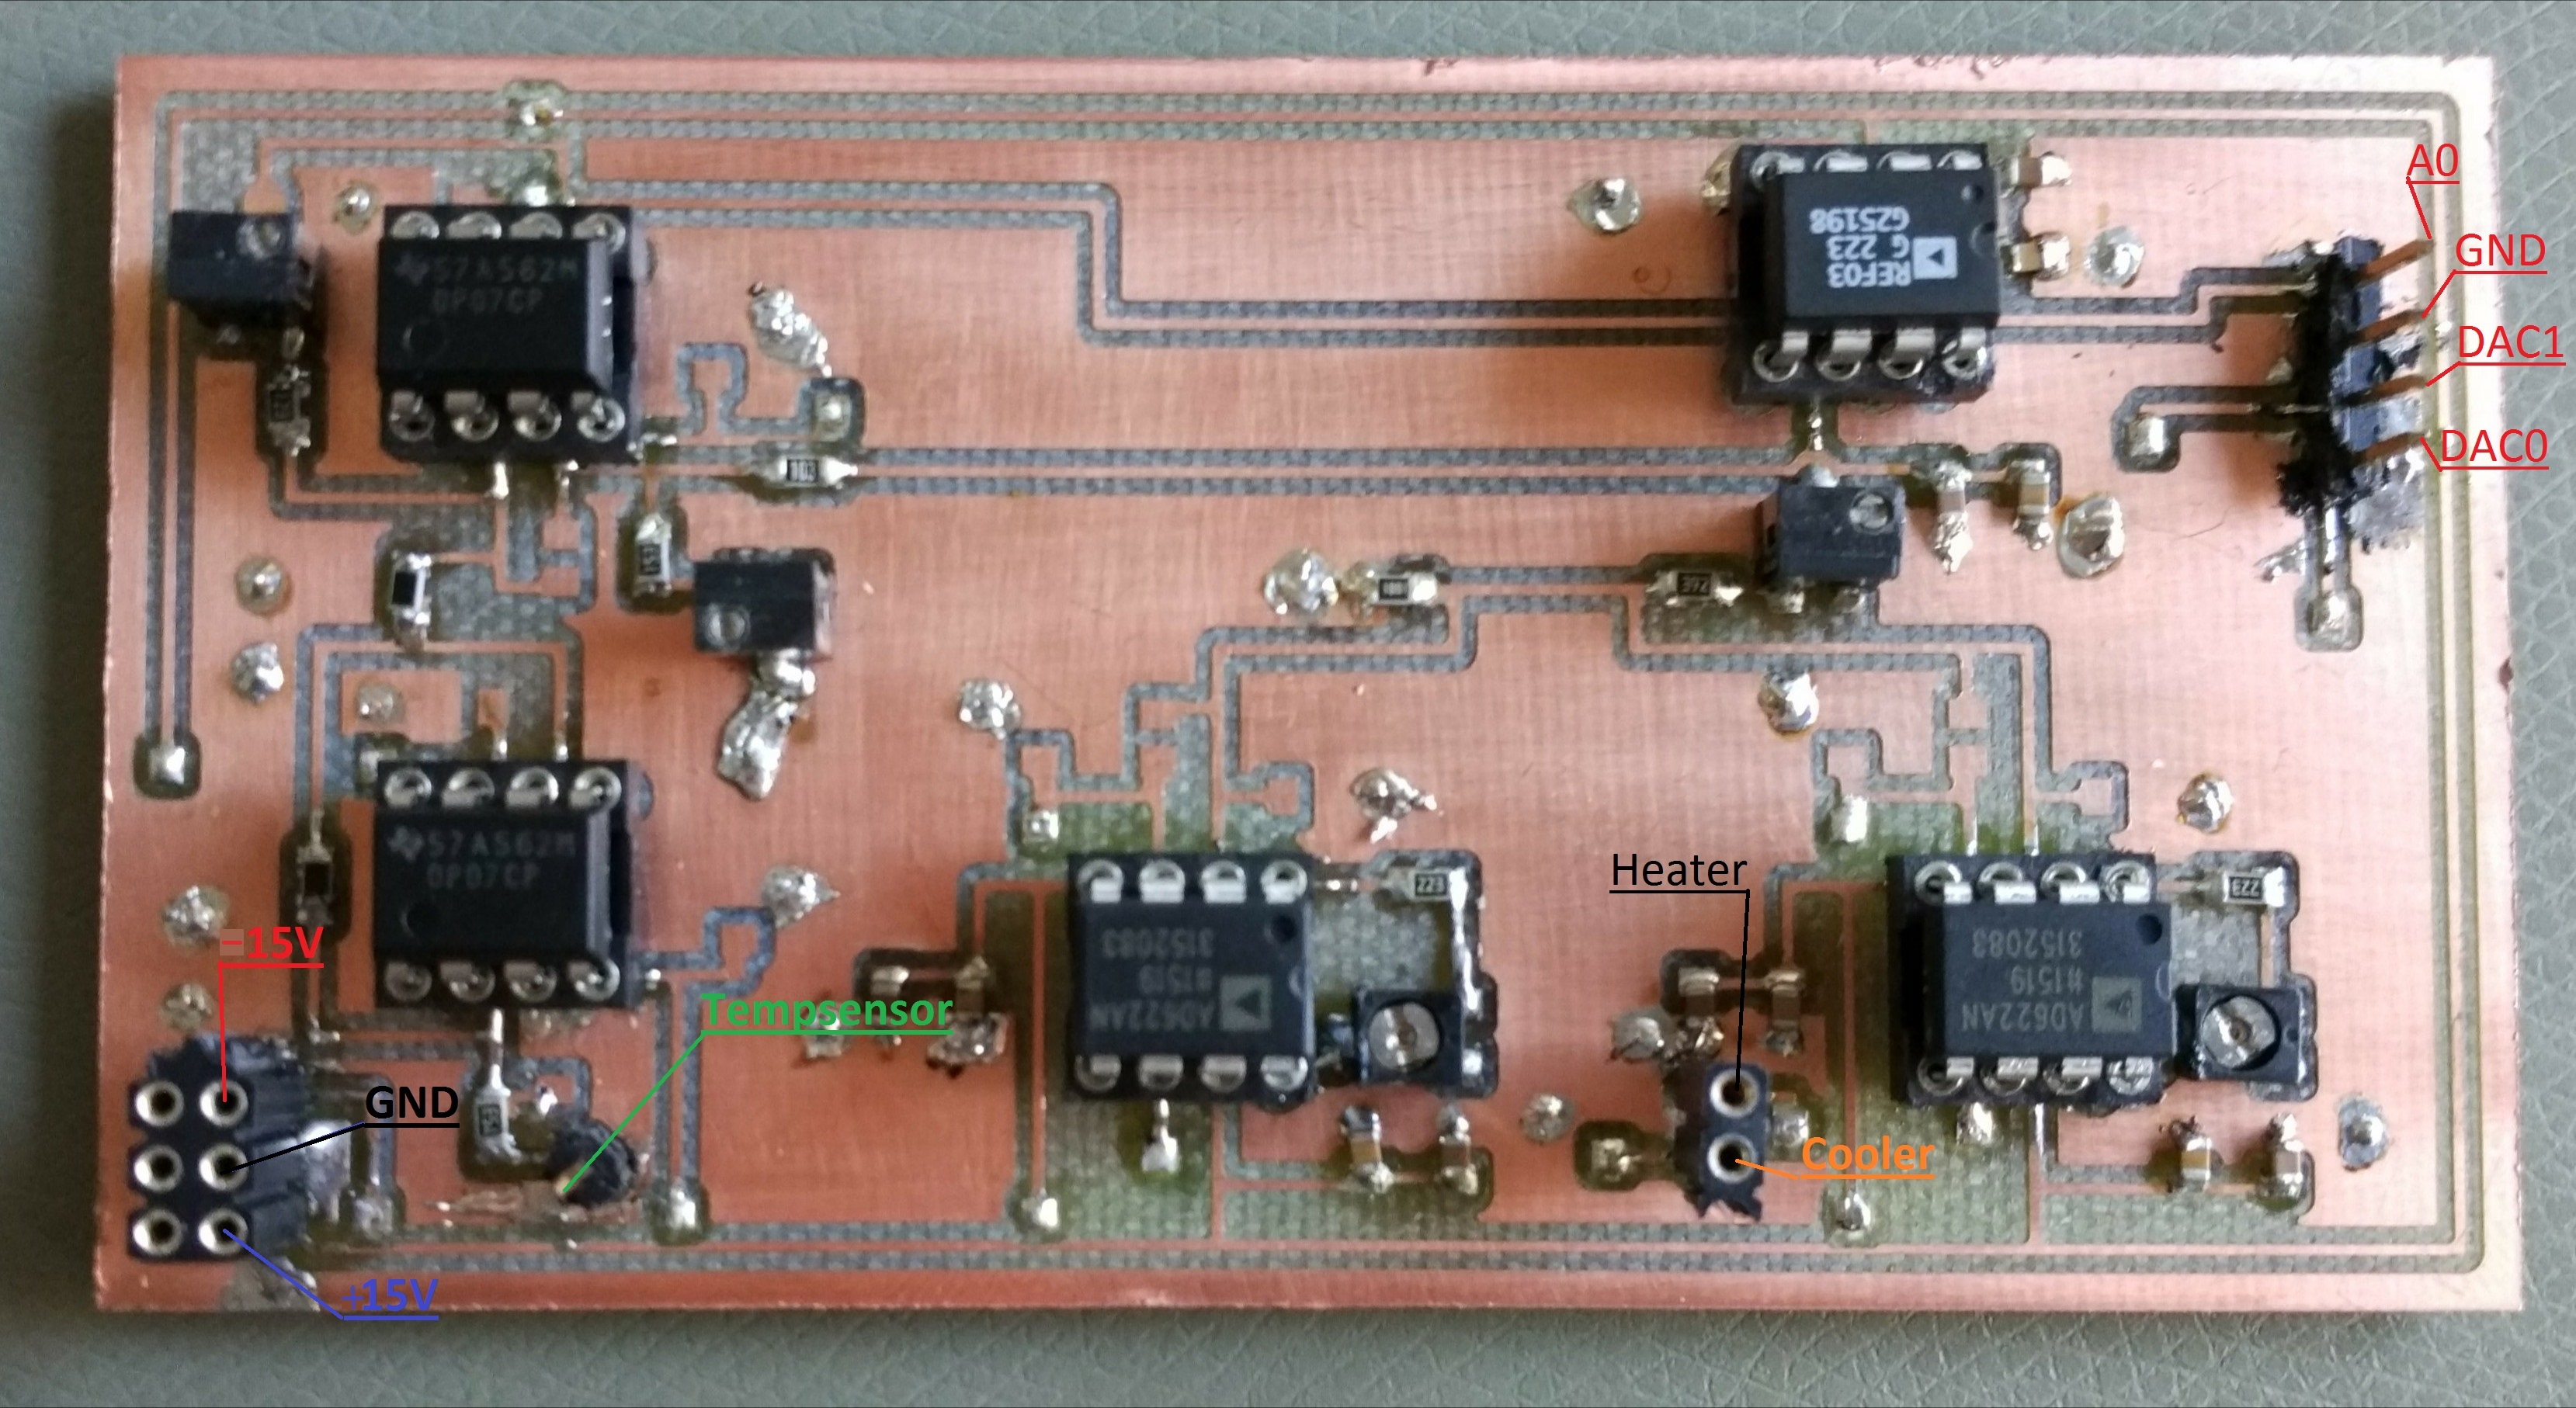
\includegraphics[width = \textwidth]{boardbild.jpg}
        \caption{Circuitboard picture}
        \label{fig5}
      \end{figure}
      \\ Notice that the header for the left AD622 was placed in the opposite
      direction, such that the marker for the top is actually on the other side
      than the top is supposed to be.\\
      Also some of the capacitances were not soldered in, on the design of the
      board they were made as a precaution.\\
      It was found that the heater/cooler cables add a capacitance which lead
      to oscillations on the temperature measurement. We added $100 \Omega$
      resistors on the heater/cooler output to resolve the issue.\\ In fig.
      \ref{fig6} we see the board connected to the Arduino with the Ethernet
      Shield 2 on top.\\
      \begin{figure}[h]
        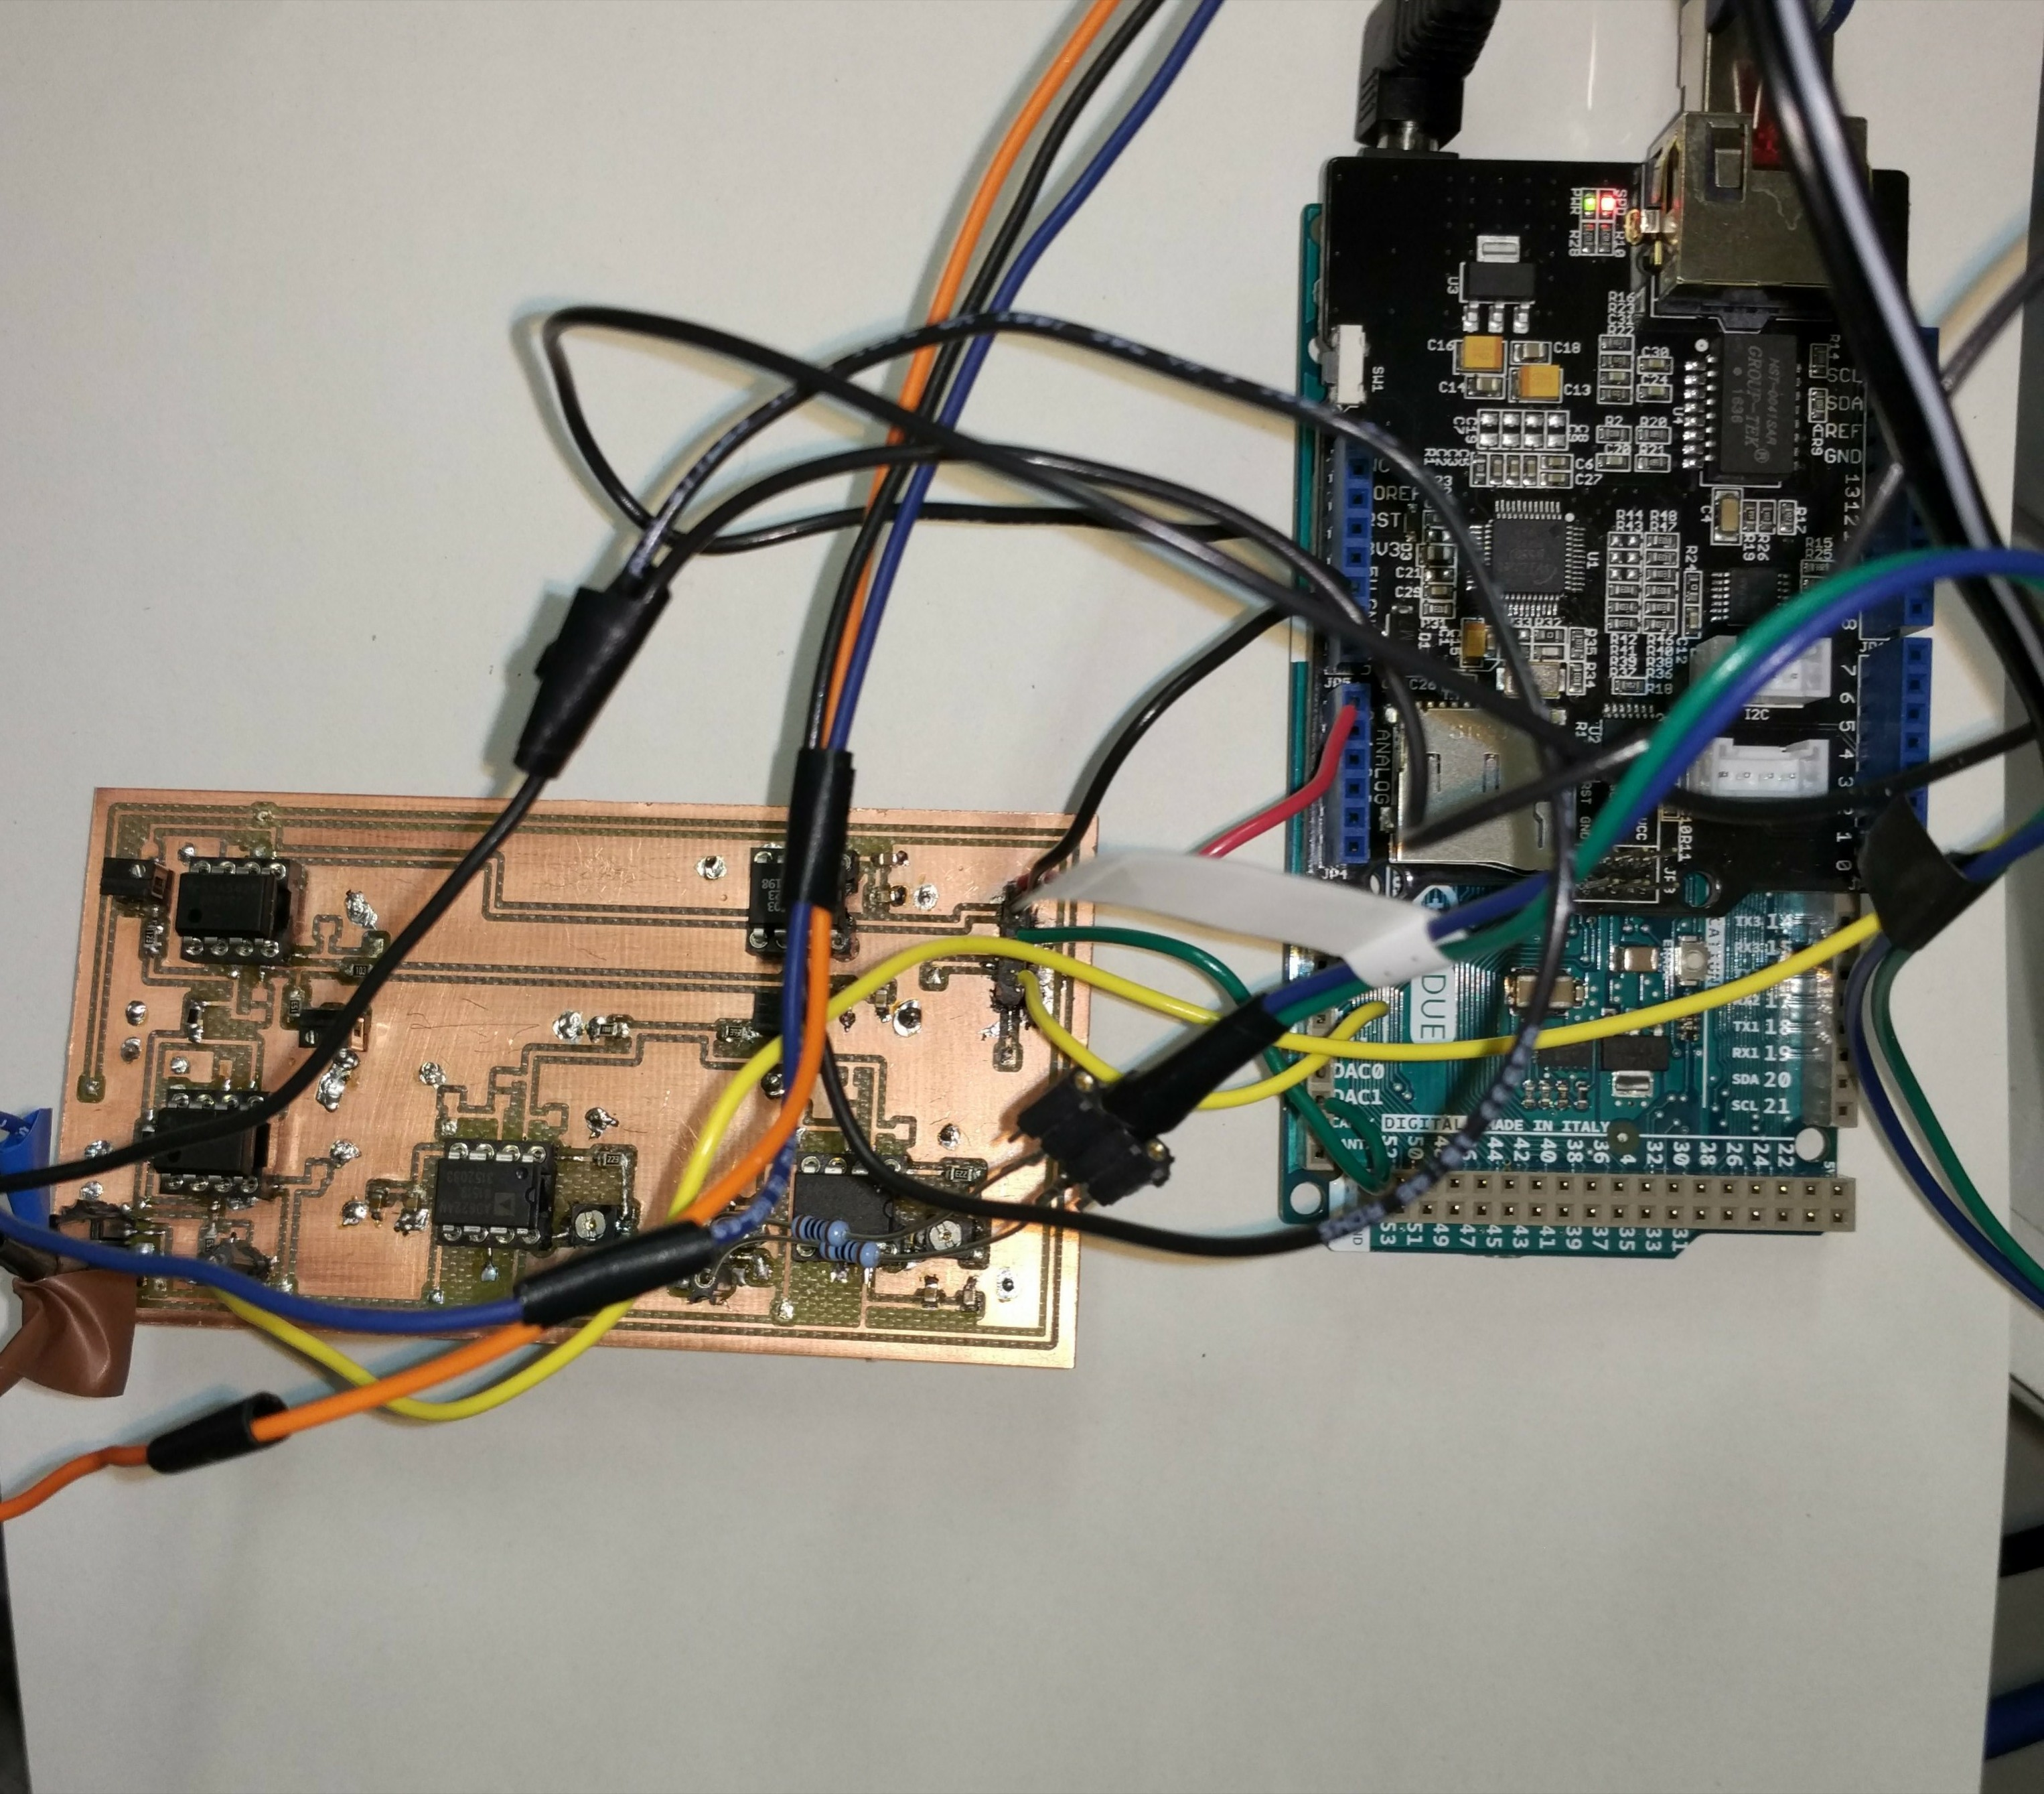
\includegraphics[width = \textwidth]{boardwitharduino.jpg}
        \caption{Board connected to Arduino}
        \label{fig6}
      \end{figure}

\end{document}
